\chapter{Unit Tests}
Zur zukünftigen Qualitätssicherung und frühzeitigen Erkennung von Fehlern wurden im Rahmen des Programmentwurfs an einigen sinnvollen Stellung exemplarische Unit Tests implementiert.
Zum Einsatz kamen hier JUnit 5, AssertJ sowie EasyMock.
\autoref{fig:uebersicht} stellt eine Übersicht über die erstellten Unit Tests dar.

\begin{figure}[H]
    \centering
    \includegraphics[width=0.5\textwidth]{Bilder/Übersicht-Unit-Tests.png}
    \caption{Übersicht über die erstellen Unit Tests}
    \label{fig:uebersicht}
\end{figure}

\section{ATRIP-Regeln}
Die ATRIP-Regeln bieten Richtlinien, die bei der Erstellung von guten und nachhaltigen Unit Tests unterstützen sollen.

\subsection{Automatic}
\label{sec:automatic}
Die Automatic Regel besagt, dass Tests eigenständig ausführbar sein sollten.
Dies inkludiert eine selbstständige Überprüfung der Ergebnisse sowie auch eine Unabhängigkeit von Nutzerinteraktion, wie etwa Eingabedialogen.
Grundsätzlich wurden alle Tests so konzipiert, dass sie gemäß den genannten Kriterien automatisch ablaufen.

Allerdings ist anzumerken, dass zwar die Durchführung aller Tests automatisiert ist, es jedoch bei den \href{https://github.com/yschiebelhut/carpool-java/blob/d0315b99dcd93e582ef60fddb185b7962bcb0076/0-carpool-java-integration/src/test/java/paypal/PayPalLinkBuilderTest.java}{Tests des PayPalLinkBuilders} zu einem Problem kommt.
Für den Einsatz der Klasse PayPalLinkBuilder wird vorausgesetzt, dass die Umgebungsvariable \code{PAYPAL\_USERNAME} gesetzt ist.
In anderen Programmiersprachen (etwa Node.js) stellt es kein Problem dar, aus einem laufenden Prozess Umgebungsvariablen zu setzen.
Somit könnte der Test diese Variable auf den erforderlichen Wert setzen.
Java hingegen betrachtet die Umgebungsvariablen, mit denen die JVM aufgerufen wurde, jedoch als immutable, weshalb sie zur Laufzeit nicht verändert werden können.
Deshalb muss der Test mit einer vorab erstellten Run-Configuration ausgeführt werden, die sicherstellt, dass die Umgebungsvariable auf den erforderlichen Wert gesetzt wird.
Dies ist zwar unpraktisch, steht einer automatisierten Testausführung aber grundsätzlich nicht im Wege.

\subsection{Thorough}
Die Thorough Regel besagt, dass gute Tests alles Notwendige abdecken sollten.
Notwendig wird hierbei durch die Rahmenbedingungen bestimmt, wie etwa Tests, die in der Vergangenheit aufgetretene Fehlerfälle abdecken.
Da im Rahmen des Programmentwurfs nur eine geringe Anzahl Tests angefertigt wurde, ist natürlich klar, dass damit nicht annähernd alle Teile des Programms abgedeckt sind.
Auch wurde das Programm für den Programmentwurf von Grund auf neu entwickelt, weshalb noch keine Bugs bekannt sind, die von Nutzern hätten gefunden werden können.
\enquote{Glücklicherweise} wurde jedoch beim Implementieren der Klasse \code{PayPalLinkBuilder} ein Bug festgestellt, der sich für die Demonstration der Regel eignet.
Bei einer ersten Implementierung gab es Probleme mit einer falschen Umwandlung von Centbeträgen, weshalb dies korrigiert und mit einem expliziten Test abgedeckt wurde (\href{https://github.com/yschiebelhut/carpool-java/blob/6d938e78763ca42270aafb8f51de4104c88e558a/0-carpool-java-integration/src/test/java/paypal/PayPalLinkBuilderTest.java#L27}{test\_generierePayPalLinkFuer1Cent}).

\subsection{Repeatable}
Gemäß der Repeatable Regel sollten Tests jederzeit automatisch durchführbar sein und dabei stets das gleiche Ergebnis liefern.
Mit den in \autoref{sec:automatic} getroffenen Maßnahmen wurde der Grundstein für Repeatable Tests bereits gelegt.
Weiterhin ist Zufall eine häufige Fehlerquelle.
Als Gegenstand einiger Tests werden Personen-Objekte erstellt.
Diese generieren bei ihrer Erstellung eine ID, welche für den weiteren Verlauf eine wichtige Bedeutung hat.
Für den (wohlgemerkt hier sehr unwahrscheinlichen) Fall, dass zufällig zweimal dieselbe ID generiert wurde, wodurch die Tests fehlschlagen würden, wurde eine \href{https://github.com/yschiebelhut/carpool-java/blob/6d938e78763ca42270aafb8f51de4104c88e558a/0-carpool-java-plugin-json/src/test/java/speicher/JsonPersonRepositoryTest.java#L132}{Einrichtung zur Prüfung} der IDs eingebaut, bevor diese im Test verwendet werden.

\subsection{Independent}
Gute Tests sollten unabhängig voneinander sein.
Das heißt, dass diese jederzeit in jeder beliebigen Zusammenstellung und Reihenfolge ausgeführt werden können.
Dies ist nur möglich, wenn Tests keine impliziten Abhängigkeiten untereinander aufbauen -- also zum Beispiel gemeinsam genutzte Datenstrukturen.
Für alle Tests wurde die Regel der Unabhängigkeit dadurch umgesetzt, das jegliche getestete Strukturen (wie zum Beispiel das \href{https://github.com/yschiebelhut/carpool-java/blob/6d938e78763ca42270aafb8f51de4104c88e558a/0-carpool-java-plugin-json/src/test/java/speicher/JsonPersonRepositoryTest.java}{JsonPersonRepository}) für jeden Test neu und in einer lokalen Variable instantiiert werden.
Somit wird eine Beeinflussung durch vorher gelaufene Tests ausgeschlossen.
Ein Test greift auch auf das Dateisystem zu.
Um hierbei eine ungewollte Abhängigkeit zu vermeiden wird für den Zugriff ein vom \href{https://github.com/yschiebelhut/carpool-java/blob/6d938e78763ca42270aafb8f51de4104c88e558a/0-carpool-java-plugin-json/src/test/java/speicher/JsonPersonRepositoryTest.java#L142}{Testframework bereitgestellter Ordner} genutzt.

\subsection{Professional}
Unit Tests sind als produktionsrelevanter Code anzusehen.
Problem ist hierbei allerdings, dass Testcode selbst keinen Tests unterliegt und fehlerhafte Tests einen Rattenschwanz an Kosten hinter sich ziehen können.
In Folge leitet die Progessional Regel ab, das Unit Tests möglichst leicht verständlich sein sollten.
Im Programmentwurf finden sich sowohl Beispiele für sehr gut strukturierte Unit Tests, als auch für verworrene und schwer zu verstehende.
Die Tests des \href{https://github.com/yschiebelhut/carpool-java/blob/6d938e78763ca42270aafb8f51de4104c88e558a/0-carpool-java-integration/src/test/java/paypal/PayPalLinkBuilderTest.java}{\code{PayPalLinkBuilder}} sind sehr kurz gehalten und folgen zudem der AAA-Normalform für Unit Tests (Arrange, Act, Assert).
Betrachtet man hingegen \href{https://github.com/yschiebelhut/carpool-java/blob/6d938e78763ca42270aafb8f51de4104c88e558a/0-carpool-java-plugin-json/src/test/java/speicher/JsonFahrgemeinschaftRepositoryTest.java#L26}{diesen Test} des \code{JsonFahrgemeinschaftRepository}, so folgt dieser auch grob der AAA-Normalform, jedoch ist er äußerst unübersichtlich geschrieben.
Es wird zur Assertion Gebrauch von der Java Reflection API gemacht und das Ergebnis mittels einer inline erstellten Map verglichen.
Selbst wenn man den Test selbst geschrieben hat, entsteht nach kurzer Zeit das Problem, diesen nicht mehr richtig lesen zu können.

\section{Code Coverage}
Für das gesamte Projekt wurde anhand der Unit Tests der Module die Testabdeckung analysiert.
Diese ist in \autoref{fig:coverage} dargestellt.
Für das gesamte Projekt liegt die Line-Coverage bei 21 \%.
Auffällig ist, dass Pakete wie \code{gui} und \code{main} keinerlei Abdeckung haben, was schlicht daran liegt, dass hierfür keine Tests geschrieben wurden.
Für das \code{model}-Paket (welches den Domain-Code enthält) hingegen wurden auch lediglich ein Test angefertigt, jedoch liegt hier die Abdeckung bei rund 55 \%.
Dies ist darauf zurückzuführen, dass Klassen aus diesem Paket in den Tests anderer Module verwendet werden.
Natürlich ist solch eine indirekte Testabdeckung eigentlich nicht wünschenswert.
Einerseits könnte man argumentieren, dass dies der Umsetzung Independent Regel entgegenwirkt, andererseits und vorrangig ergibt sich das Problem, dass die Domain-Schicht aktuell fast ausschließlich von Code aus höheren Schichten getestet wird.
Diese Schichten sind kurzlebig und könnten theoretisch jederzeit obsolet wäre, wodurch die Domain-Schicht praktisch von einem Moment auf den anderen nicht mehr von Tests abgedeckt wäre.

\begin{figure}[H]
    \centering
    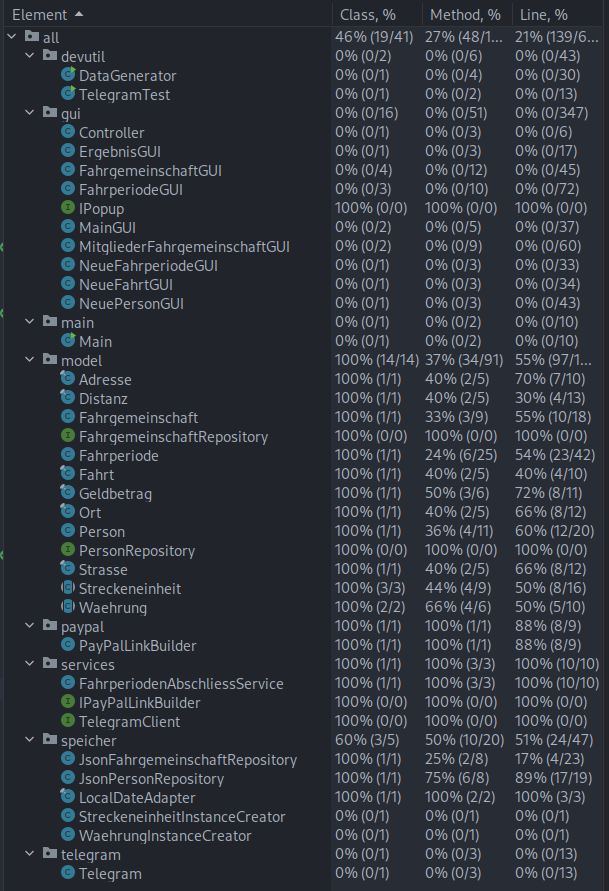
\includegraphics[width=0.5\textwidth]{Bilder/Coverage.png}
    \caption{Coverage-Analyse des Projekts}
    \label{fig:coverage}
\end{figure}

\section{Einsatz von Mocks}
Mocks werden bei Unit Tests eingesetzt, um Abhängigkeiten während eines Tests zu ersetzen.
So hängt beispielsweise das Ergebnis eines Tests nicht von einer externen Datenbank ab.
Weiterhin könnte so auch einer Kopplung, wie im letzten Absatz beschrieben, entgegengewirkt werden.

Im Programmentwurf wurden in mehreren Tests Mocks eingesetzt.
Besonders gut zu sehen ist dies in den \href{https://github.com/yschiebelhut/carpool-java/blob/6d938e78763ca42270aafb8f51de4104c88e558a/0-carpool-java-plugin-json/src/test/java/speicher/LocalDateAdapterTest.java}{Tests des \code{LocalDateAdapters}}.
Hier wird bei beiden Tests mittels Mocks vermieden, dass ein echter JsonReader/-Writer erstellt werden muss, der wiederum einen Ein-/Ausgabestream voraussetzt -- beispielsweise aus einer Datei.